\section{Method}
\label{sec: method}



The AR diffusion distillation pipelines reviewed in Sec.~\ref{sec:bg-distillation} have achieved strong results in chunk-wise (typically 3 latent frames) 4-step AR generation, but two questions remain open. First, none of them has been validated in more aggressive low-latency regimes---in particular, \emph{frame-wise AR generation with as few as 1--2 sampling steps}---which would better realize the low-latency promise of real-time interactive generation. Second, the existing few-step initialization strategy, ODE distillation, requires the teacher to generate full PF-ODE trajectories for every training datum; this is structurally expensive and makes systematic exploration of harder regimes costly. In this section we address both. We first show that no existing initialization strategy is satisfactory in our target regime (Sec.~\ref{sec:necessity}); we then propose causal consistency distillation as a principled and scalable substitute for causal ODE distillation (Sec.~\ref{sec:substitute}); finally, we extend our method to action-conditioned world model generation (Sec.~\ref{sec:application}). The overview of our method and its relation to previous works are shown in Fig.~\ref{fig:overall}.

\subsection{The Necessity of Few-Step AR Student Initialization}
\label{sec:necessity}

Since asymmetric DMD is highly sensitive to its few-step student initialization~\cite{zhu2026causal}, we begin by examining whether existing initialization strategies suffice in our target regime. In recent works, three options have been proposed: (i) distilling a few-step AR student from a \emph{bidirectional} teacher via ODE distillation, as in CausVid~\cite{yin2025slow} and Self Forcing~\cite{huang2025self}; (ii) skipping few-step distillation entirely and using the multi-step AR diffusion model directly, as in LiveAvatar~\cite{huang2025live} and WorldPlay~\cite{sun2025worldplay}; and (iii) distilling a few-step AR student from an \emph{AR} teacher via ODE distillation, as in Causal Forcing~\cite{zhu2026causal}. We compare these three candidates as the autoregressive unit shrinks from chunk-wise to frame-wise and the sampling step count drops from 4 to 1. As shown in Fig.~\ref{fig:multi-step}, we find that all three fall short for complementary reasons: one is architecturally misaligned, one is too weak, and one is too costly to scale. This motivates an initialization that is simultaneously \emph{AR}, \emph{few-step}, and \emph{scalable}, as we now establish.

\newcommand{\leftfigwidth}{0.67\linewidth}
\newcommand{\rightfigwidth}{0.25\linewidth}
\newcommand{\figxshift}{-0.02\linewidth}
\newcommand{\figgap}{0.05\linewidth}

\begin{figure}[t]
  \centering
    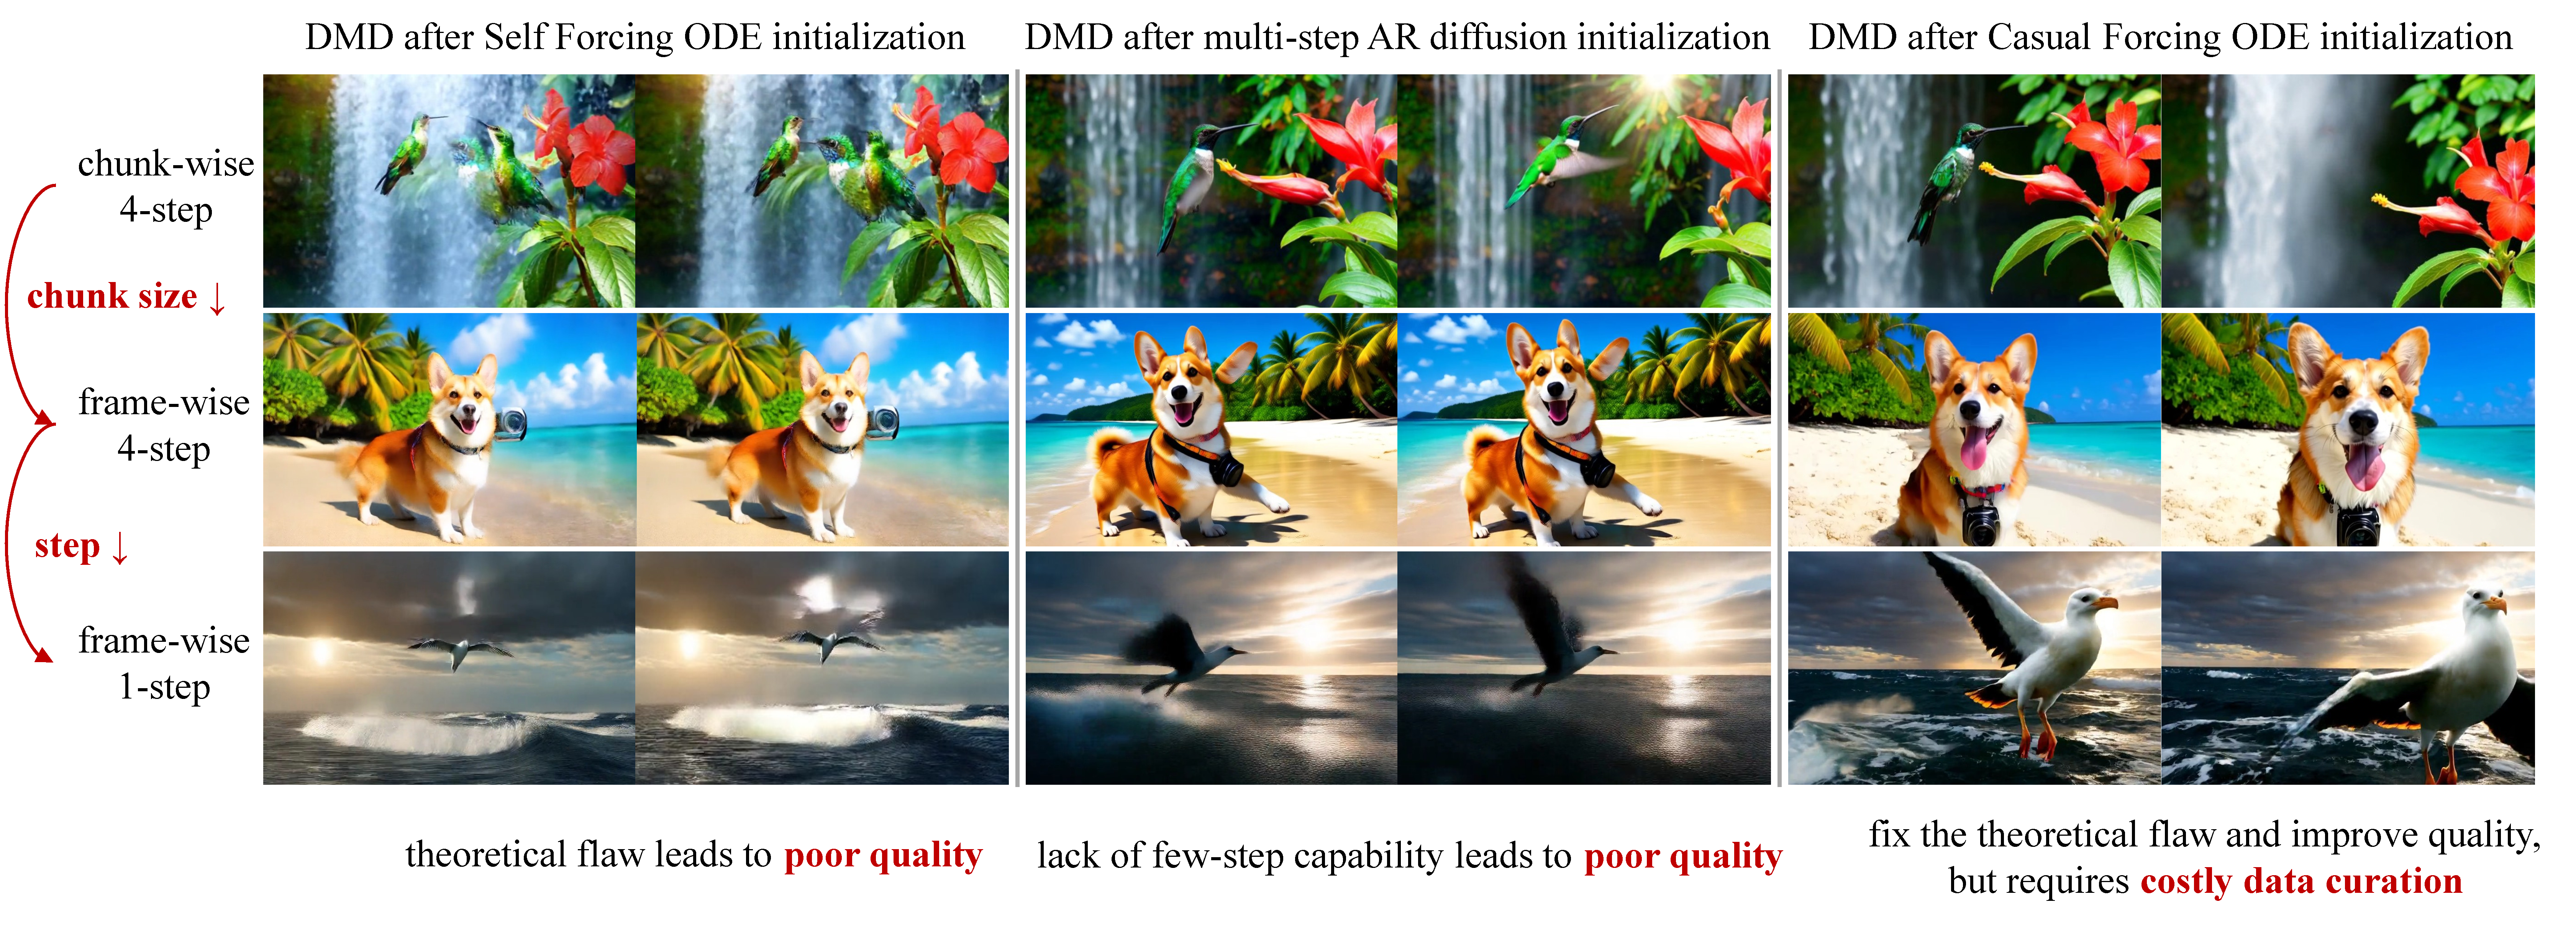
\includegraphics[width=\linewidth]{Figures/multi-step-a.pdf}
  \caption{\textbf{Performance of existing initialization methods after DMD.} Self Forcing ODE initialization and multi-step AR diffusion initialization leads to poor quality and degrade as the setting becomes more aggressive, while Causal Forcing's causal ODE initialization performs well but is costly and therefore difficult to scale.}
  \label{fig:multi-step}
\end{figure}



\paragraph{ODE initialization with a bidirectional teacher is misaligned.}

The first candidate uses \emph{ODE distillation with a bidirectional teacher}, which is the initialization mechanism behind CausVid~\cite{yin2025slow} and Self Forcing~\cite{huang2025self}. As Causal Forcing~\cite{zhu2026causal} shows, this choice violates the \emph{frame-level injectivity} required by an AR student---the same noisy frame can correspond to multiple clean frames under different future contexts---so ODE distillation no longer recovers the AR flow map but instead collapses toward the conditional expectation $\E[\vx_0^i \mid \vx_t^i, \vx_t^{<i}, t]$, producing a blurred and poorly aligned initialization. This mismatch becomes more damaging in our frame-wise low-step settings, where the student must repeatedly roll out from its own imperfect history. Quantitatively, asymmetric DMD with Self-Forcing-style initialization already collapses in the chunk-wise 4-step setting, becomes even worse in the frame-wise 4-step setting, and eventually catastrophically breaks down in the frame-wise 1-step setting, as illustrated in Fig. \ref{fig:multi-step}(column 1). \emph{ODE initialization with a bidirectional teacher} is therefore fundamentally flawed and not a viable foundation for low-latency AR diffusion distillation.

\paragraph{Multi-step AR diffusion initialization degrades sharply in aggressive settings.} Using the multi-step AR diffusion model directly as the student initialization yields consistently weaker results than explicit few-step distillation, and this gap widens as we move toward lower-latency generation. As shown in Fig.~\ref{fig:multi-step}(column 2 vs. column 3), the gap is moderate under chunk-wise generation, larger under frame-wise 4-step, and largest under frame-wise 1-step, where the model nearly collapses. The reason is structural: reducing the chunk size increases the number of AR calls needed to generate a video, while reducing the sampling step count increases the approximation error within each call. These two effects compound during self-rollout, amplifying exposure bias. In this sense, asymmetric DMD acts as a refiner rather than a complete trainer: if the initialization lacks few-step capability, DMD inherits an optimization burden it cannot reliably absorb.


\paragraph{Casual ODE initialization with an AR teacher works, but is difficult to scale.}
Causal Forcing~\cite{zhu2026causal} addresses the architectural mismatch of Self-Forcing-style ODE initialization by replacing the bidirectional teacher \emph{with an AR teacher} and performing causal ODE distillation between AR models. This produces a well-aligned few-step initialization and leads to strong chunk-wise 4-step results after asymmetric DMD, as illustrated in Fig. \ref{fig:multi-step}(column 3). Its limitation is not correctness but scalability: each training datum requires the AR teacher to generate a full multi-step PF-ODE trajectory (e.g., 48 steps per sample); these paired trajectories must be stored offline; and they must be regenerated whenever the teacher, data distribution, or chunk-size configuration changes. Worse, the cost grows with task difficulty: harder regimes typically demand more training data and longer trajectories, compounding the bottleneck.
At our 80K-video scale, this data curation along with the training costs roughly $11{,}600$ A800-GPU hours and $1{,}900$\,GiB of additional storage, as quantified in Tab. \ref{tab:ablation}. Thus, causal ODE initialization works in principle but imposes a structural scaling bottleneck that limits its practical reach.

Taken together, the three existing options leave us with no satisfactory initialization for asymmetric DMD in aggressive low-latency regimes: one is architecturally misaligned, one lacks few-step capability, and one is too costly to scale. We therefore need an initialization that is simultaneously \emph{AR}, \emph{few-step}, and \emph{scalable}. 

\subsection{Causal Forcing++: Causal CD as a Principled and Scalable Substitute for Causal ODE Initialization}
\label{sec:substitute}

Sec.~\ref{sec:necessity} established that the initialization of asymmetric DMD should be simultaneously \emph{AR}, \emph{few-step}, and \emph{scalable}, and that causal ODE distillation~\cite{zhu2026causal} satisfies only the first two. Our key observation is that causal ODE distillation and causal consistency distillation (CD) shares the same learning target: the flow map (or the consistency function) of the AR teacher. Building on this equivalence, we propose causal CD as the few-step AR student initialization. We show that this substitution is principled---sharing the learning target of causal ODE distillation---and brings two practical advantages: it eliminates the offline-trajectory bottleneck and yields a stronger initialization via a smaller per-step optimization gap. We refer to the resulting pipeline as \textbf{\textit{Causal Forcing++}}.


\paragraph{Causal ODE distillation shares the same target as causal consistency distillation.}
Causal ODE distillation~\cite{zhu2026causal} collects intermediate states $\vx_t^i$ and corresponding clean outputs $\vx_0^i$ along the PF-ODE trajectory of the AR diffusion teacher, and trains the student by MSE regression with teacher forcing:
\begin{align}
    \theta^*=\arg\min_\theta \mathbb{E}_{\vx_{\mathrm{gt}}^{<i},\, t,\, i,\, \vx_t^i}\left[\,\|G_\theta(\vx_t^i,\vx_{\mathrm{gt}}^{<i}, t)-\vx_0^i\|^2\,\right].
\end{align}
The minimizer of this objective is the AR-conditional flow map of the teacher,
\begin{align}
    \vf_\phi:(\vx_t^i,\,\vx_{\mathrm{gt}}^{<i},\,t)\mapsto \vx_0^i,
\end{align}
which maps $\vx_t^i$ at any time $t$ to the PF-ODE sample $\vx_0^i$ of the teacher diffusion model $\phi$ at $t=0$. 
Recognizing $\vf_\phi$ as the AR-conditional analog of the consistency function~\cite{song2023consistency,song2023improved,wang2024phased,lu2024simplifying,zheng2025large}, we lift the standard CD objective to the AR setting via teacher forcing:
\begin{align}
\label{eq:causal-cd}
\theta^*=\arg\min_\theta \mathbb{E}_{\vx_\text{gt},\,\vepsilon,\,t,\,i}\Big[w(t)\,d\big(G_\theta(\vx_t^i,\vx_\text{gt}^{<i}, t),\; G_{\theta^-}(\hat{\vx}^i_{t-\Delta t},\vx_\text{gt}^{<i}, t-\Delta t)\big)\Big],
\end{align}
where $\vx_t^i$ is obtained from the ground-truth $\vx_\text{gt}^i$ via the forward diffusion process, $\hat{\vx}^i_{t-\Delta t}$ is obtained by a single ODE step from $\vx_t^i$ using the AR teacher conditioned on the ground-truth prefix $\vx_\text{gt}^{<i}$, $\theta^-$ is the EMA of $\theta$ with stop-gradient, $w(\cdot)$ is a timestep-dependent weight, and $d(\cdot,\cdot)$ is a distance under a pre-defined norm. Under the flow-matching parameterization of Sec.~\ref{sec: diffusion},
\begin{align}
G_\theta(\vx_t^i,\vx_\text{gt}^{<i},t) = \vx_t^i - t\,\vv_\theta(\vx_t^i,\vx_\text{gt}^{<i},t),
\end{align}
where $\vv_\theta$ is the neural network. Following standard CD analysis~\cite{song2023consistency}, the error between the optimal model $G_{\theta^*}$ and the target flow map $f_\phi$ (namely the consistency function) is bounded by the numerical error of the ODE solver and is therefore negligible:
\begin{align}
    \mathrm{sup}||f_\phi(\vx_t^i, \vx_{\mathrm{gt}}^{<i},t) - G_{\theta^*}(\vx_t^i, \vx_{\mathrm{gt}}^{<i},t)||_2 = \gO((\Delta t)^p),
\end{align}
where $\Delta t$ denotes the maximum difference between adjacent timesteps, and the ODE solver is $p$-th order accurate.

In other words, causal ODE distillation and causal CD share the same target; they differ only in how that target is approached---ODE distillation regresses to it via large jumps from $t$ to $0$ on pre-generated trajectories, while CD enforces it locally between adjacent timesteps on real data. This equivalence motivates causal CD as a principled substitute for causal ODE distillation.

\begin{figure}[t]
  \centering
  \hspace*{\figxshift}%
  \begin{subfigure}[t]{\leftfigwidth}
    \centering
    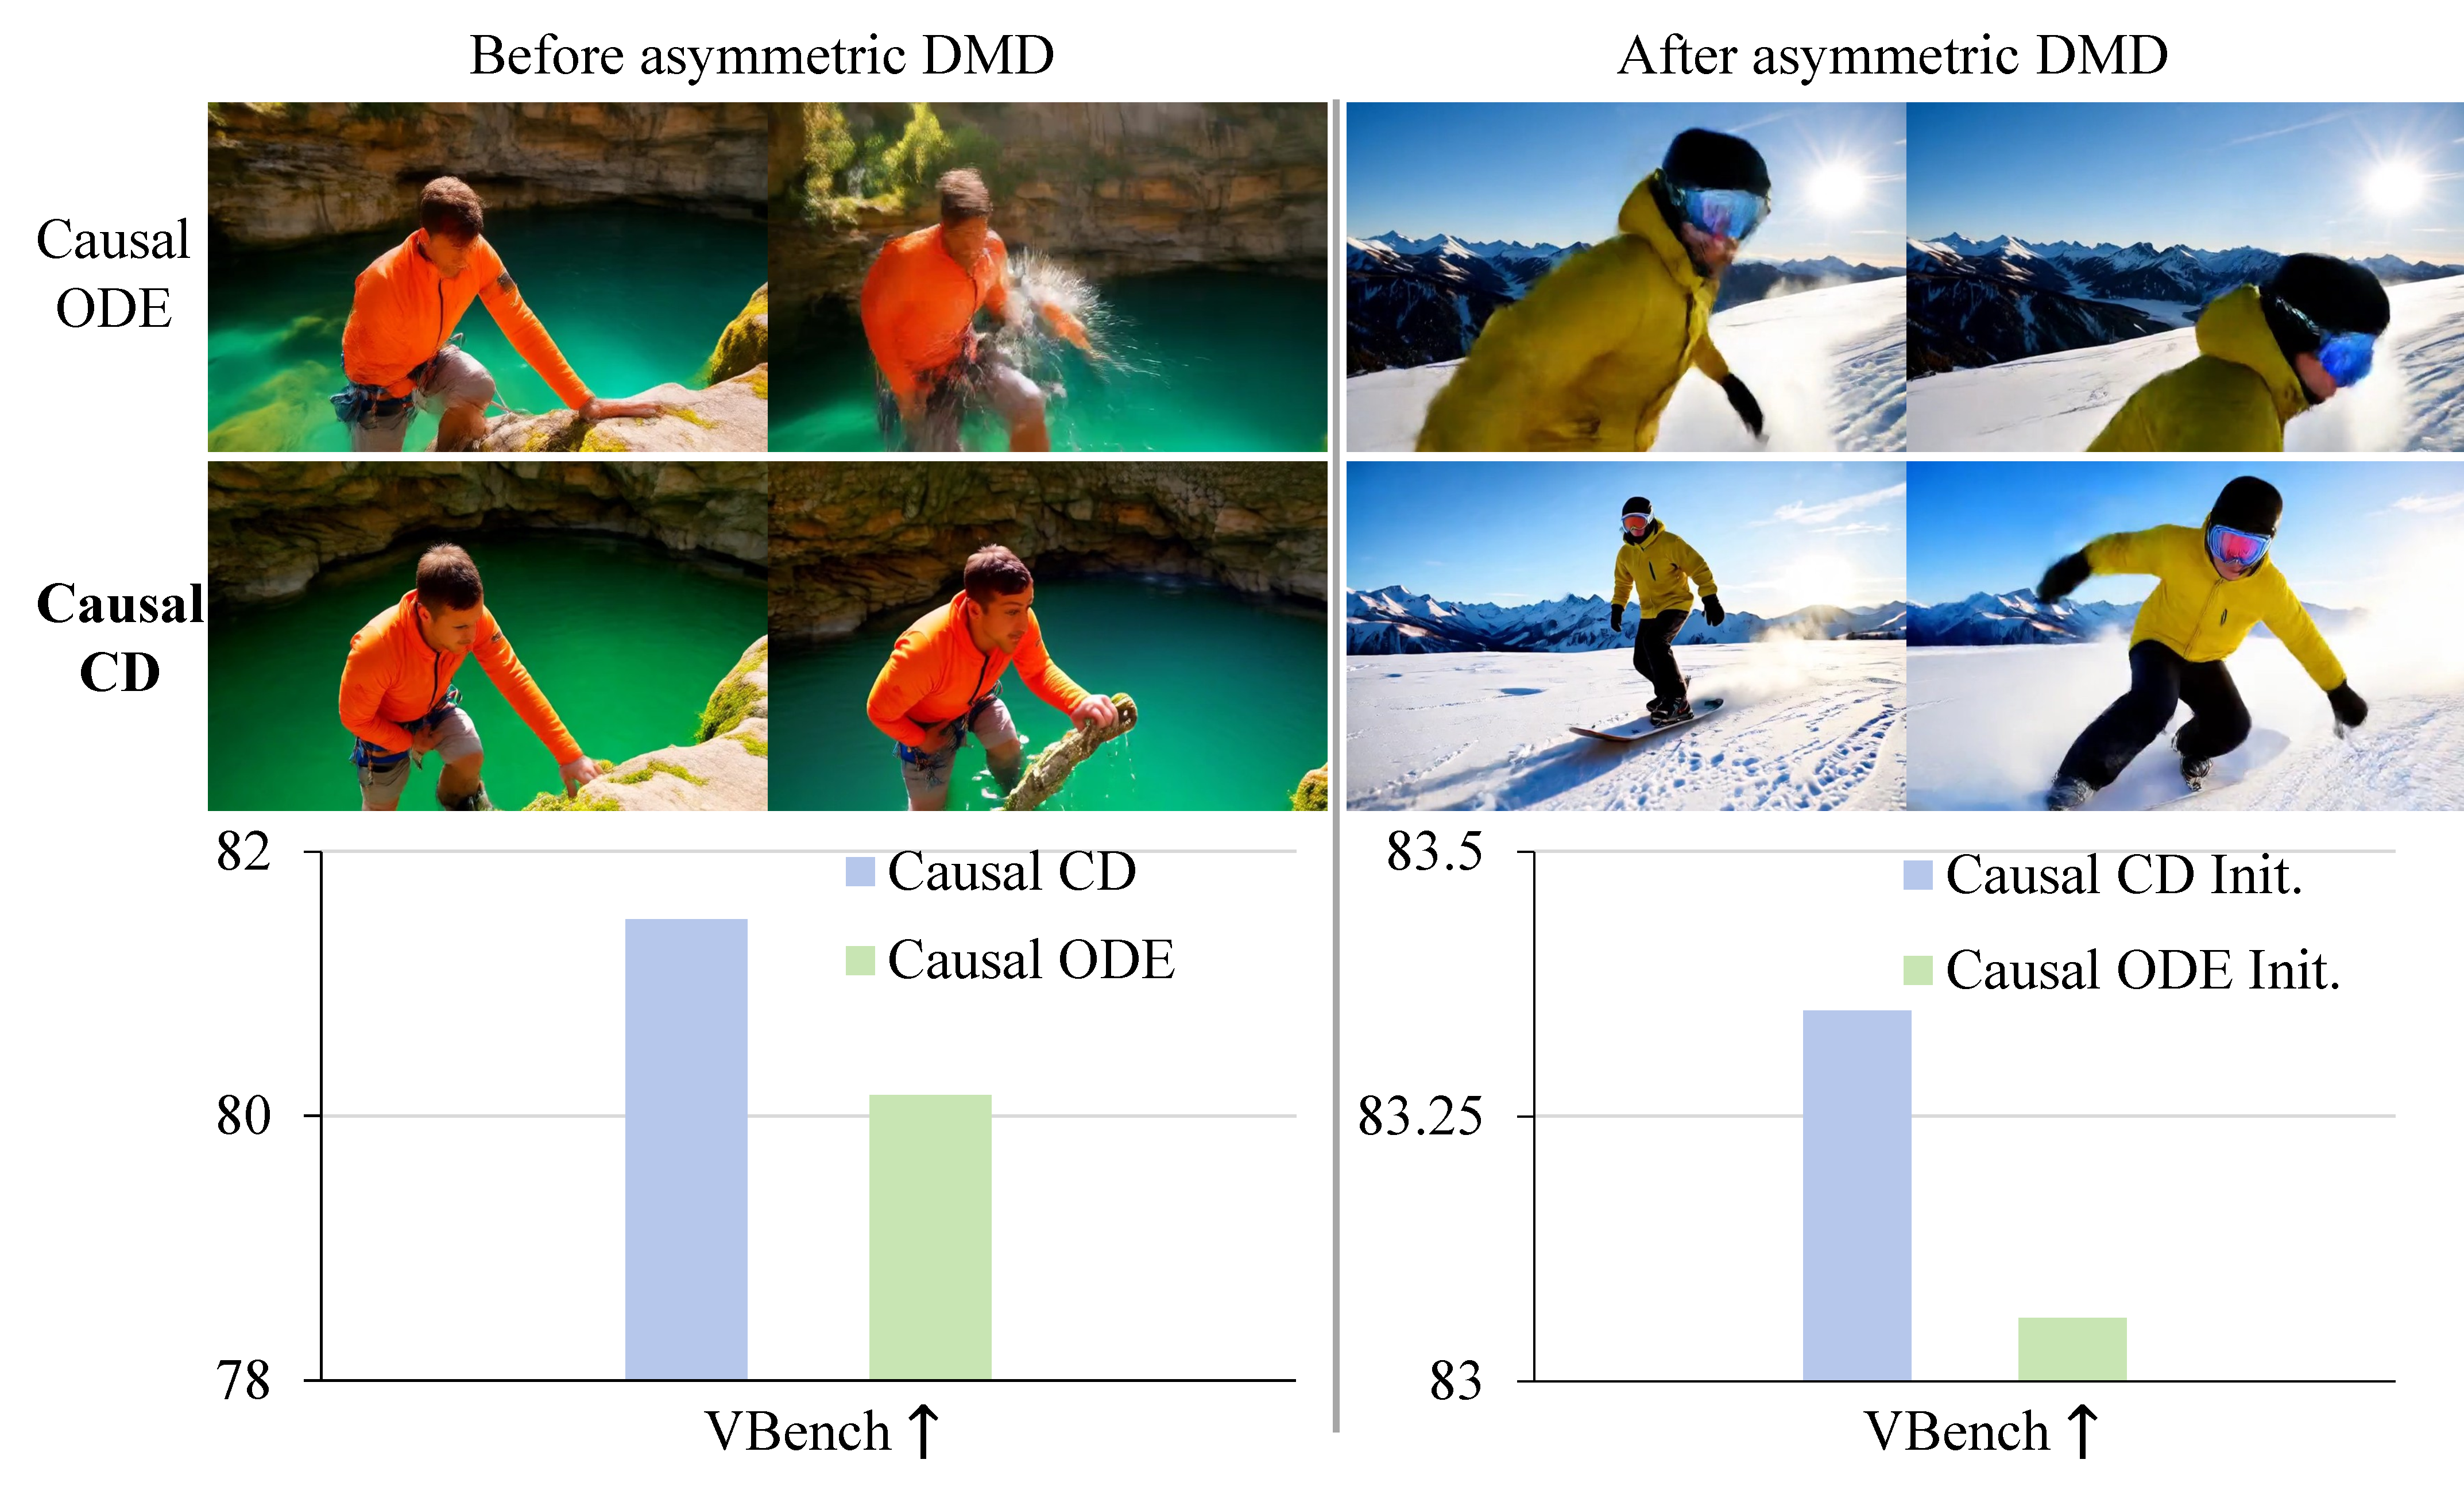
\includegraphics[width=\linewidth]{Figures/causal-cd-a.pdf}
    \caption{\footnotesize Performance comparison.
Causal CD achieves higher VBench scores than causal ODE both when directly evaluated at Stage~2 and when used as the initialization for Stage~3, while also producing videos with better visual quality. Init. denotes initialization.
}
    \label{fig:causal-cd-a}
  \end{subfigure}%
  \hspace{\figgap}%
  \begin{subfigure}[t]{\rightfigwidth}
    \centering
    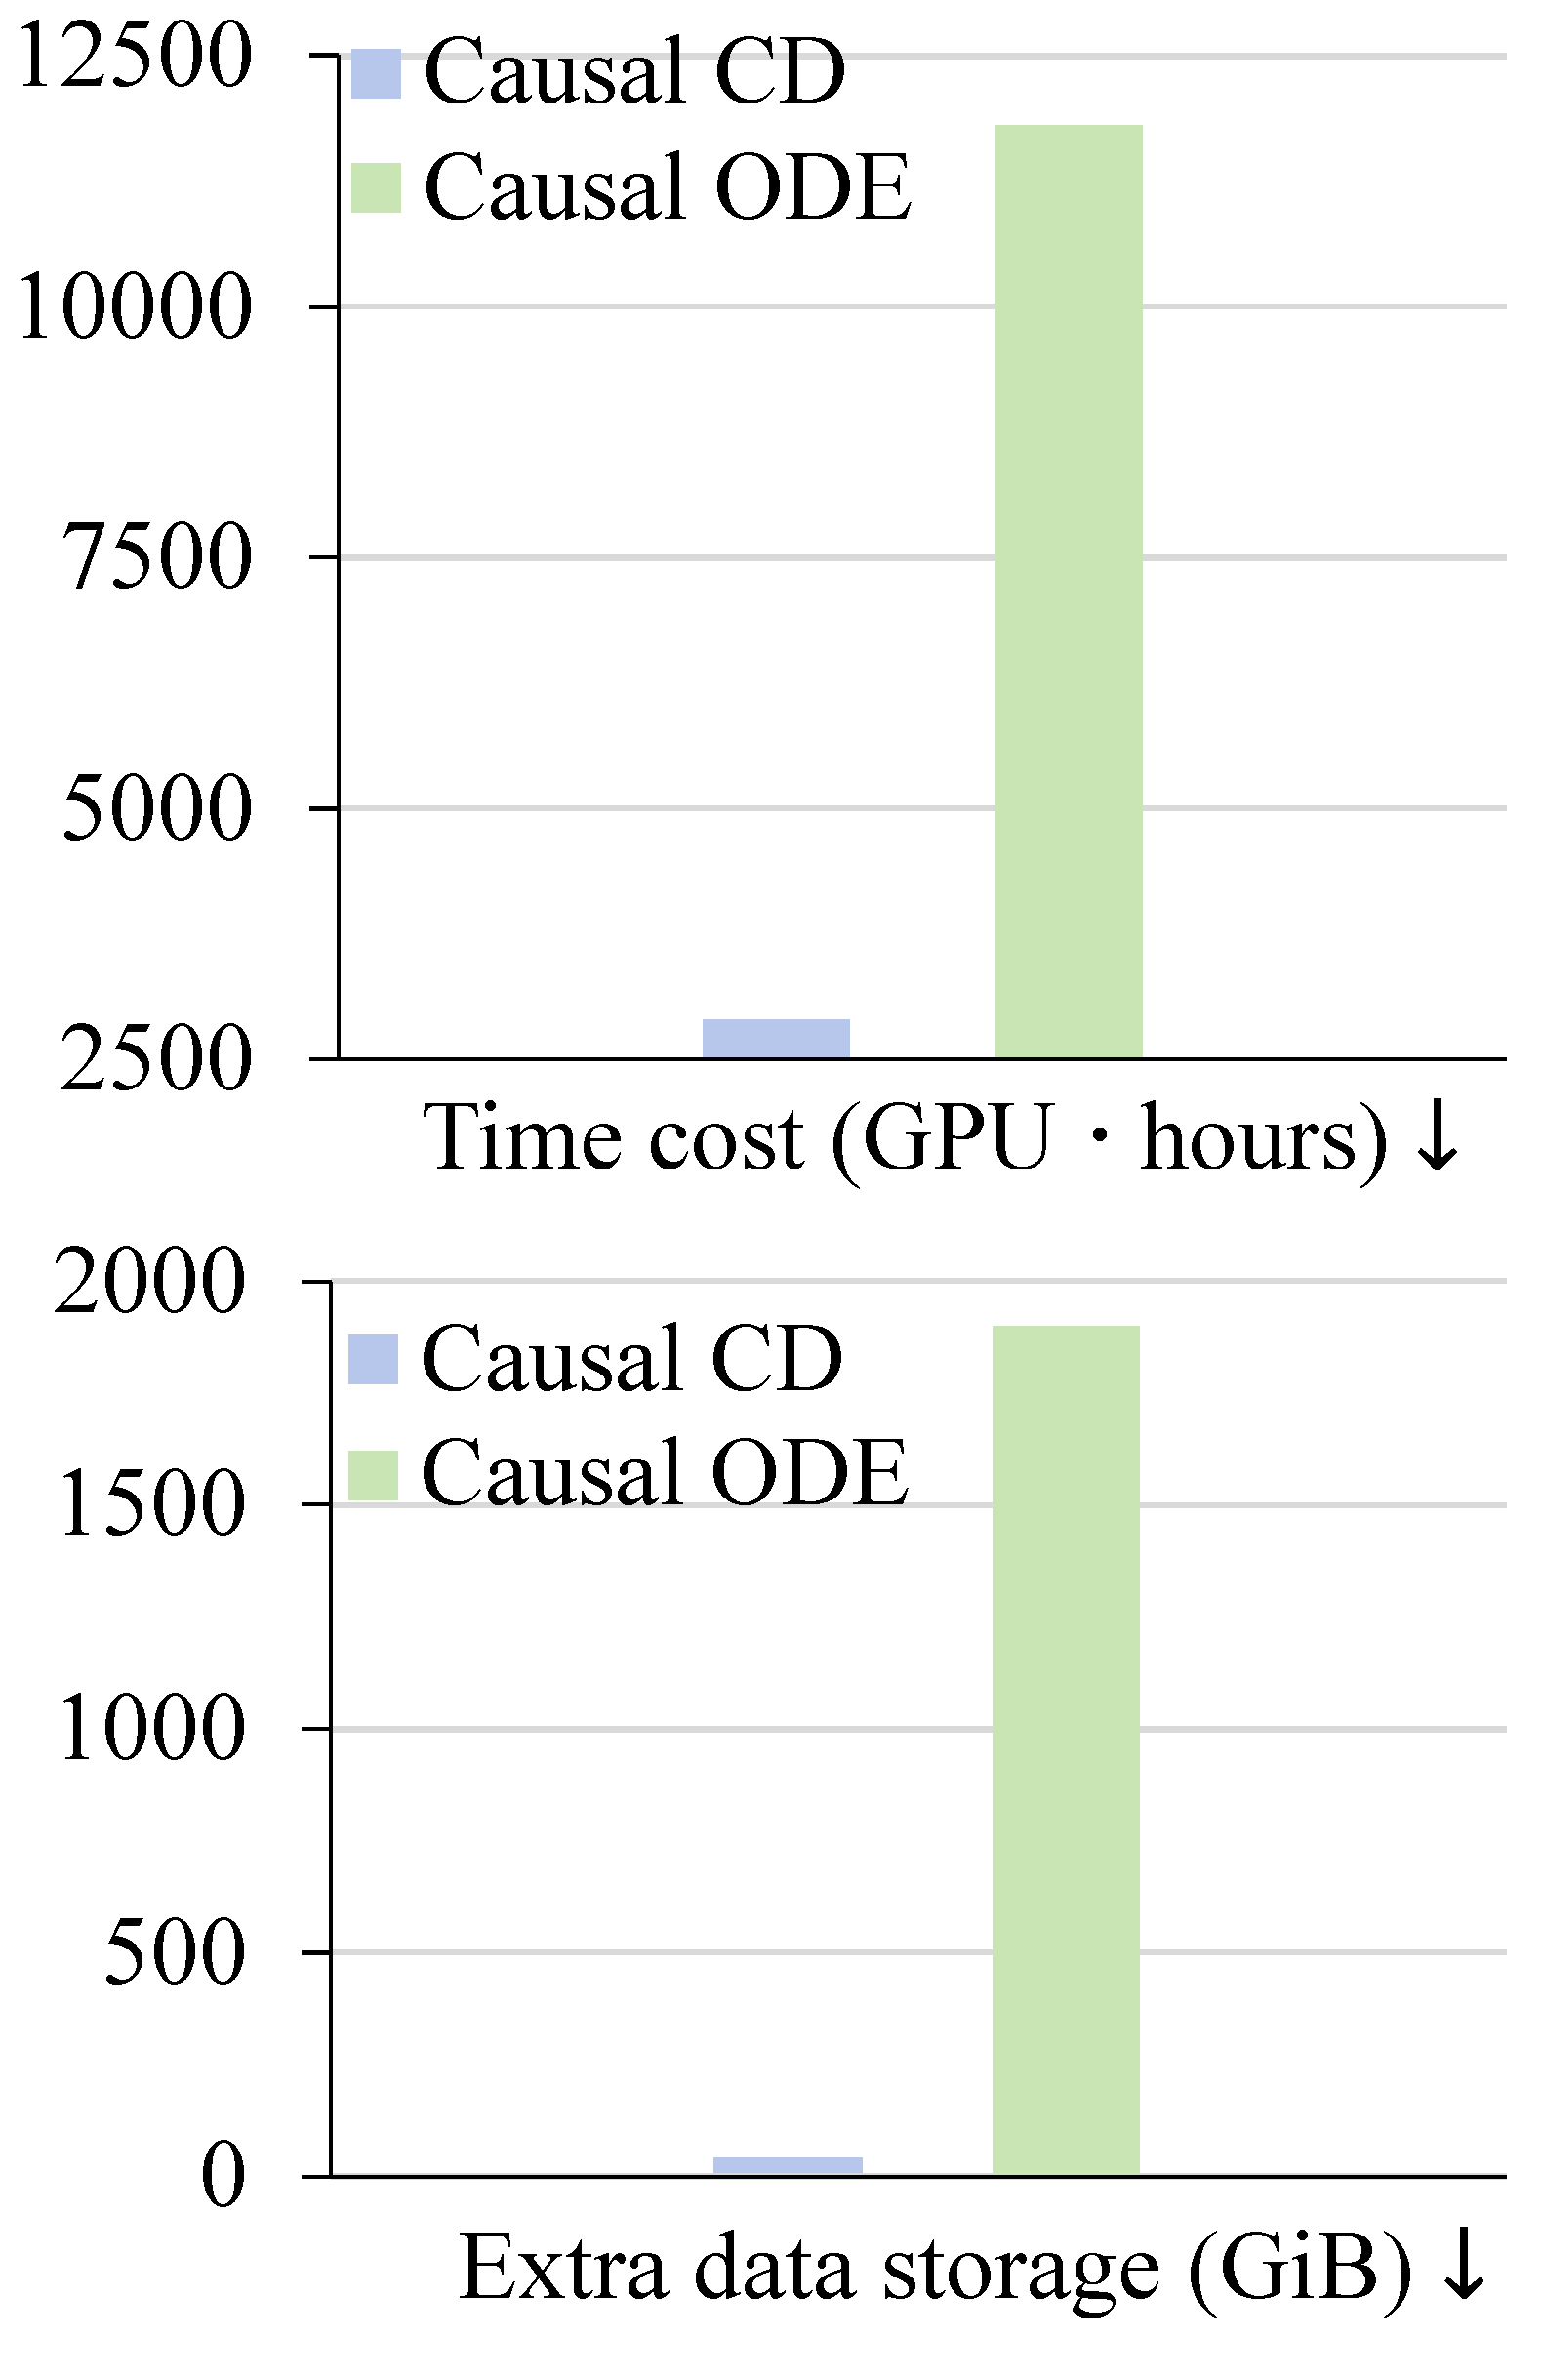
\includegraphics[width=\linewidth]{Figures/causal-cd-b.pdf}
    \caption{\footnotesize Training-efficiency.
Causal CD dramatically reduces training time and requires no extra storage.
}
    \label{fig:causal-cd-b}
  \end{subfigure}
\vspace{-.25cm}
  \caption{\textbf{Performance and efficiency comparison between causal CD and causal ODE.}
Causal CD outperforms causal ODE, while subsequently improving training efficiency in time and storage.}
  \label{fig:cd-is-better-than-ode}
\end{figure}

\paragraph{Causal CD is more efficient and yields a stronger initialization.} Beyond principled equivalence, Causal CD delivers two practical advantages over causal ODE distillation. \textbf{(1) Efficiency.} 
Causal ODE distillation requires the teacher to pre-generate a full multi-step PF-ODE trajectory for every training datum (e.g., 48 steps), store the paired trajectories offline, and regenerate them whenever the teacher or data distribution changes. Causal CD requires only \emph{one} teacher ODE step per training iteration, performed online on ground-truth videos. At our 80K-video scale (Fig.~\ref{fig:cd-is-better-than-ode}(b)), this reduces the data curation and training cost from $\sim$$11{,}600$ to $\sim$$2{,}900$ A800-GPU hours ($\sim$$4\times$ speedup) and the auxiliary storage from $\sim$$1{,}900$\,GiB to zero. \textbf{(2) Quality.} Causal ODE distillation regresses $\vx_t^i$ to $\vx_0^i$ across the entire $t \to 0$ interval, asking the student to bridge a large gap in one step. Causal CD instead pairs $\vx_t^i$ with $\hat{\vx}^i_{t-\Delta t}$ between adjacent timesteps, reducing the per-step gap to $\Delta t$ and yielding an easier optimization target---consistent with prior observations in bidirectional distillation~\cite{liu2023instaflow}. Empirically (Fig.~\ref{fig:cd-is-better-than-ode}(a)), causal CD matches or surpasses causal ODE distillation on VBench~\cite{huang2024vbench} both at the end of Stage~2 and after the asymmetric DMD stage. These advantages are structural properties of the local-pairing scheme and apply uniformly across chunk-wise and frame-wise configurations.

\paragraph{Causal Forcing++.} Putting these pieces together, our pipeline inherits Stage~1 (teacher forcing AR diffusion training) and Stage~3 (asymmetric DMD with self-rollout) from Causal Forcing~\cite{zhu2026causal}, and replaces its Stage~2 with the causal CD objective of Eq.~(\ref{eq:causal-cd}). We refer to this pipeline as \textbf{\textit{Causal Forcing++}}. In summary, Causal Forcing++ improves over prior AR diffusion distillation along two complementary axes. Relative to Self Forcing~\cite{huang2025self}, whose ODE initialization from a bidirectional teacher violates frame-level injectivity and degenerates to a conditional-expectation target, Causal Forcing++ is both \emph{correct}---targeting the correct AR flow map---and \emph{more efficient}, since causal CD avoids offline trajectory generation entirely. Relative to Causal Forcing~\cite{zhu2026causal}, whose causal ODE initialization recovers the correct target but is bottlenecked by offline trajectory generation, Causal Forcing++ is both \emph{more efficient} and \emph{higher-quality}, owing to the smaller per-step optimization gap of local consistency pairing.

\subsection{Application to Action-Conditioned World Models}
\label{sec:application}

We further showcase the applicability of our pipeline to action-conditioned world model generation. Following the Genie3-style~\cite{genie3} camera-pose conditioning paradigm, we instantiate a chunk-wise 4-step generator based on Wan2.1-1.3B, using camera poses as the action signal. The pipeline involves three stages: (i) constructing a camera-pose-annotated training dataset with WorldPlay~\cite{sun2025worldplay}; (ii) finetuning Wan2.1-1.3B into a bidirectional camera-pose-conditioned diffusion model by injecting pose information via PRoPE~\cite{li2026cameras}; and (iii) distilling this bidirectional model with Causal Forcing++ into an interactive action-conditioned world model. Qualitative results are shown in Fig.~\ref{fig:action}, and full demos are provided on the project page. Further reducing the action-conditioned variant to the frame-wise 2-step setting for fully real-time interaction is left for future work.

\newcommand{\ablationfigwidth}{\linewidth}

\begin{figure}
  \centering

  \begin{subfigure}{\ablationfigwidth}
    \centering
    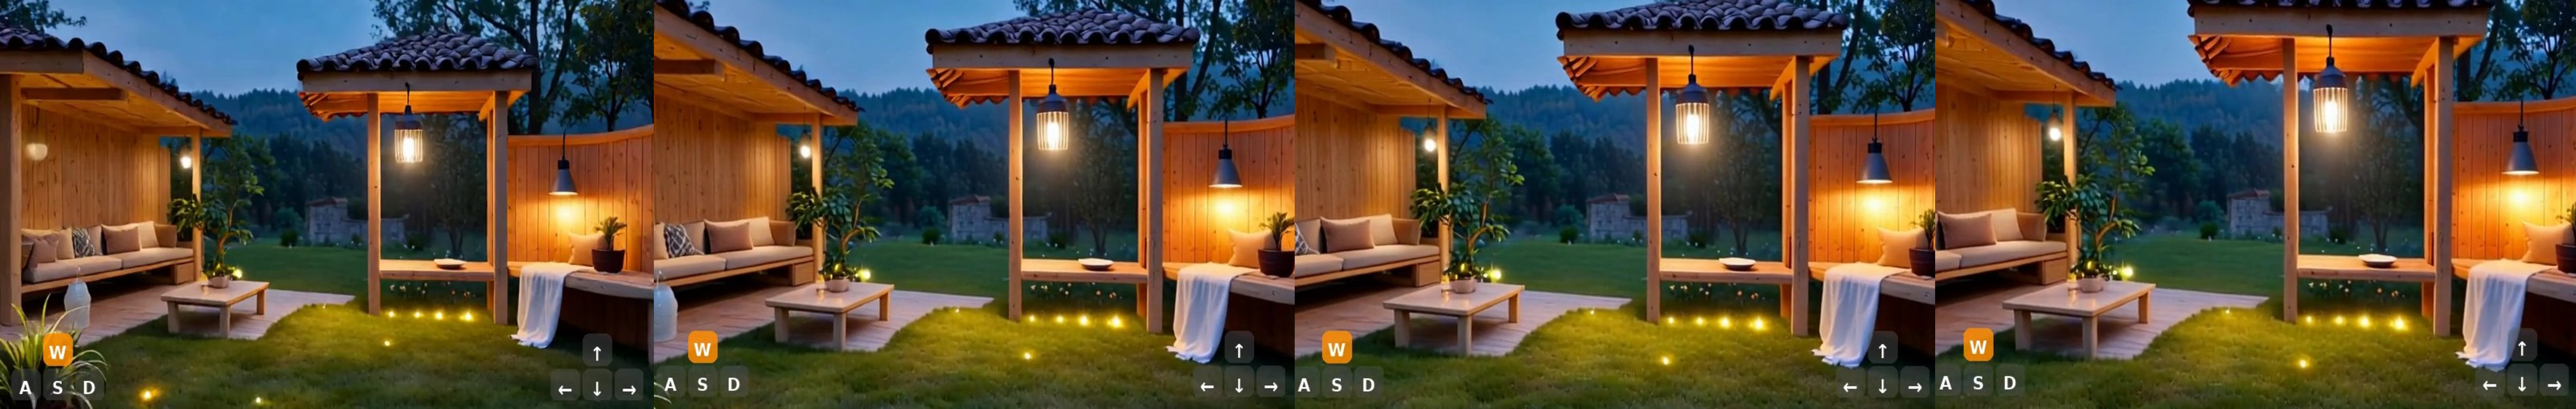
\includegraphics[width=\linewidth]{Figures/W19.pdf}
    \caption{\footnotesize Action: moving forward continuously.}
  \end{subfigure}

  \vspace{0.5em}

  \begin{subfigure}{\ablationfigwidth}
    \centering
    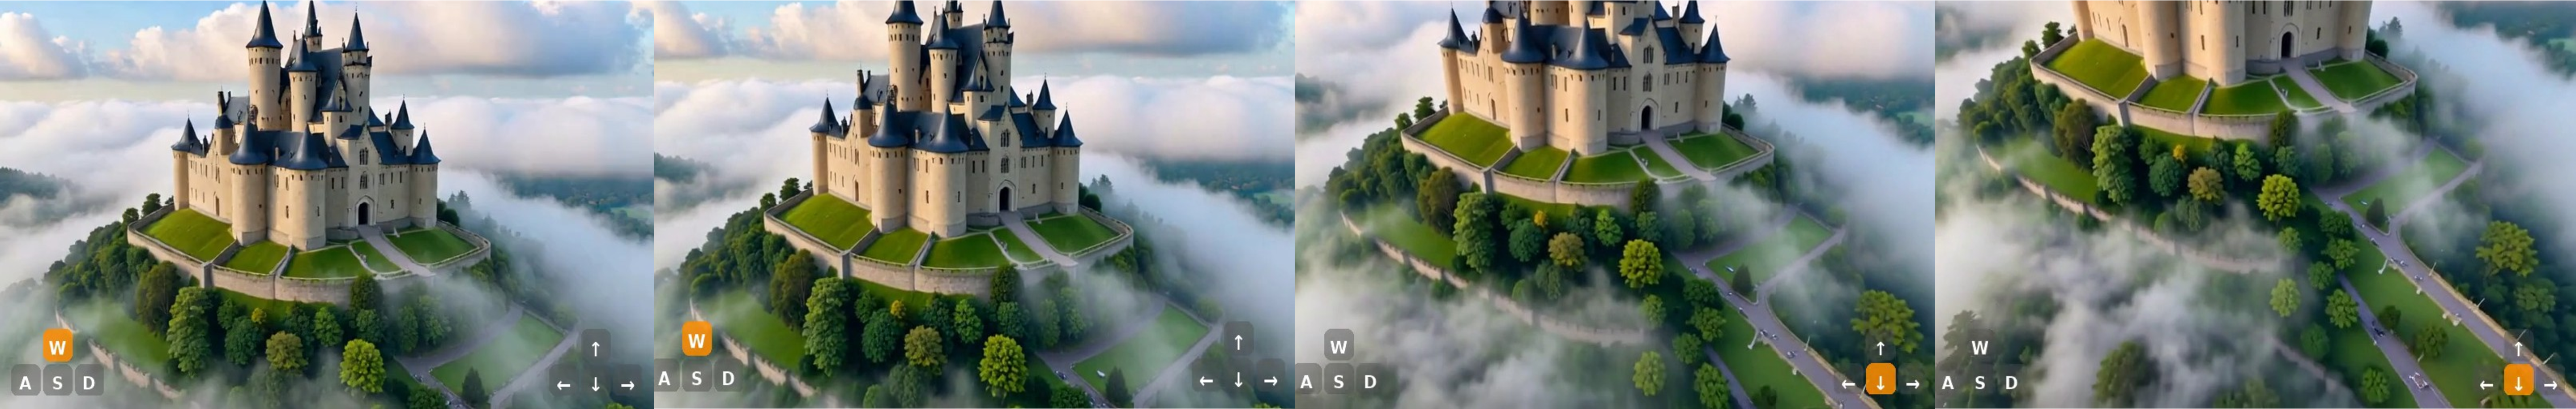
\includegraphics[width=\linewidth]{Figures/WK.pdf}
    \caption{\footnotesize Action: move forward first, then tilt the camera downward.}
  \end{subfigure}


  \caption{\textbf{Application of Causal Forcing++ to the action-conditioned world model.} Causal Forcing++ enables efficient, high-quality distillation from a bidirectional model to a low-latency AR model, thereby enabling interactive generation toward a Genie3-style world model.}
  \label{fig:action}

\end{figure}

\subsection{Further Discussion: Whether Causal Score Distillation Yields Strong Initialization}

\label{sec: causal dmd}

Since causal consistency distillation has been shown to provide a strong few-step initialization above, a natural question is whether its counterpart in step distillation, namely score distillation~\cite{wang2023prolificdreamer,luo2023diff,yin2024one}, can also serve this role. Given that score distillation often yields higher quality than consistency distillation in bidirectional distillation~\cite{yin2024one,yin2024improved,zheng2025large}, this appears promising. In this section, we examine whether causal score distillation actually works.


\begin{figure}[t]
  \centering
  \hspace*{\figxshift}%
  \begin{subfigure}[t]{\leftfigwidth}
    \centering
    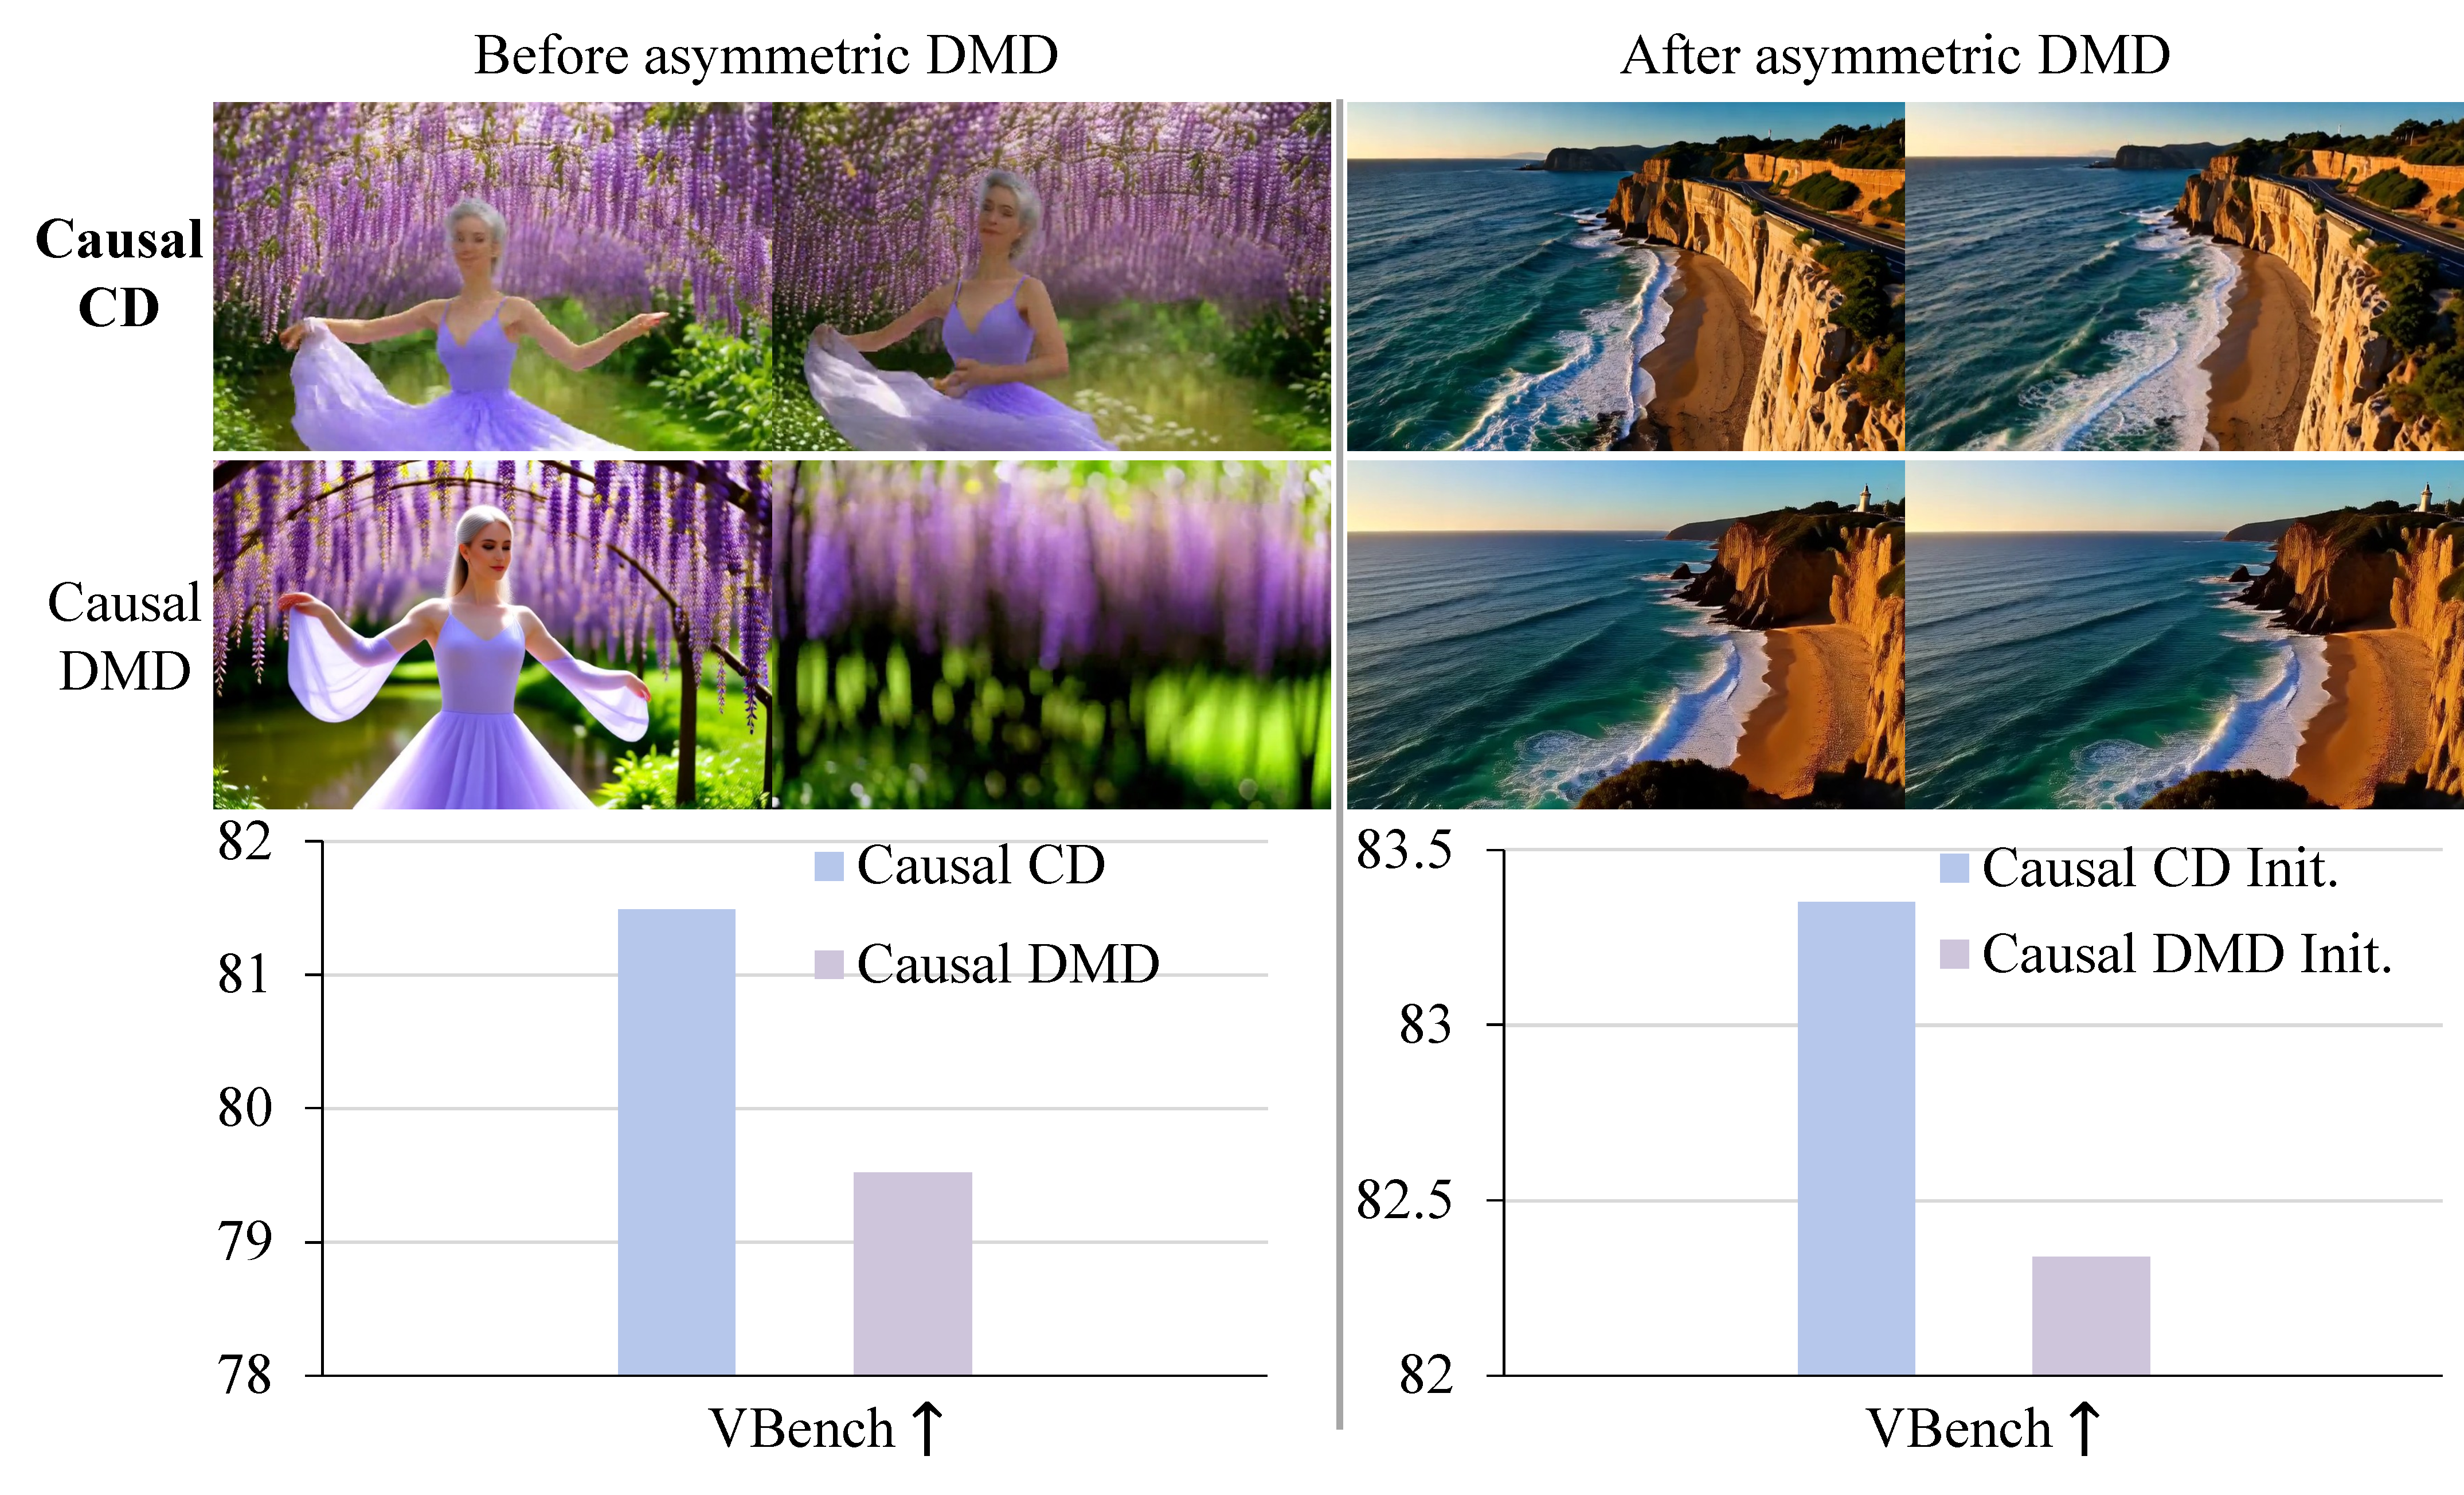
\includegraphics[width=0.95\linewidth]{Figures/causal-dmd-a.pdf}
    \caption{\footnotesize Performance comparison. Causal DMD yields lower VBench scores than causal CD both when directly evaluated after Stage 2 and when used as the initialization for Stage 3. Although causal DMD produces sharper early frames, its quality rapidly drifts during autoregressive rollout, leading to severe exposure bias. Init. denotes initialization.}
    \label{fig:causal-dmd-a}
  \end{subfigure}%
  \hspace{\figgap}%
  \begin{subfigure}[t]{\rightfigwidth}
    \centering
    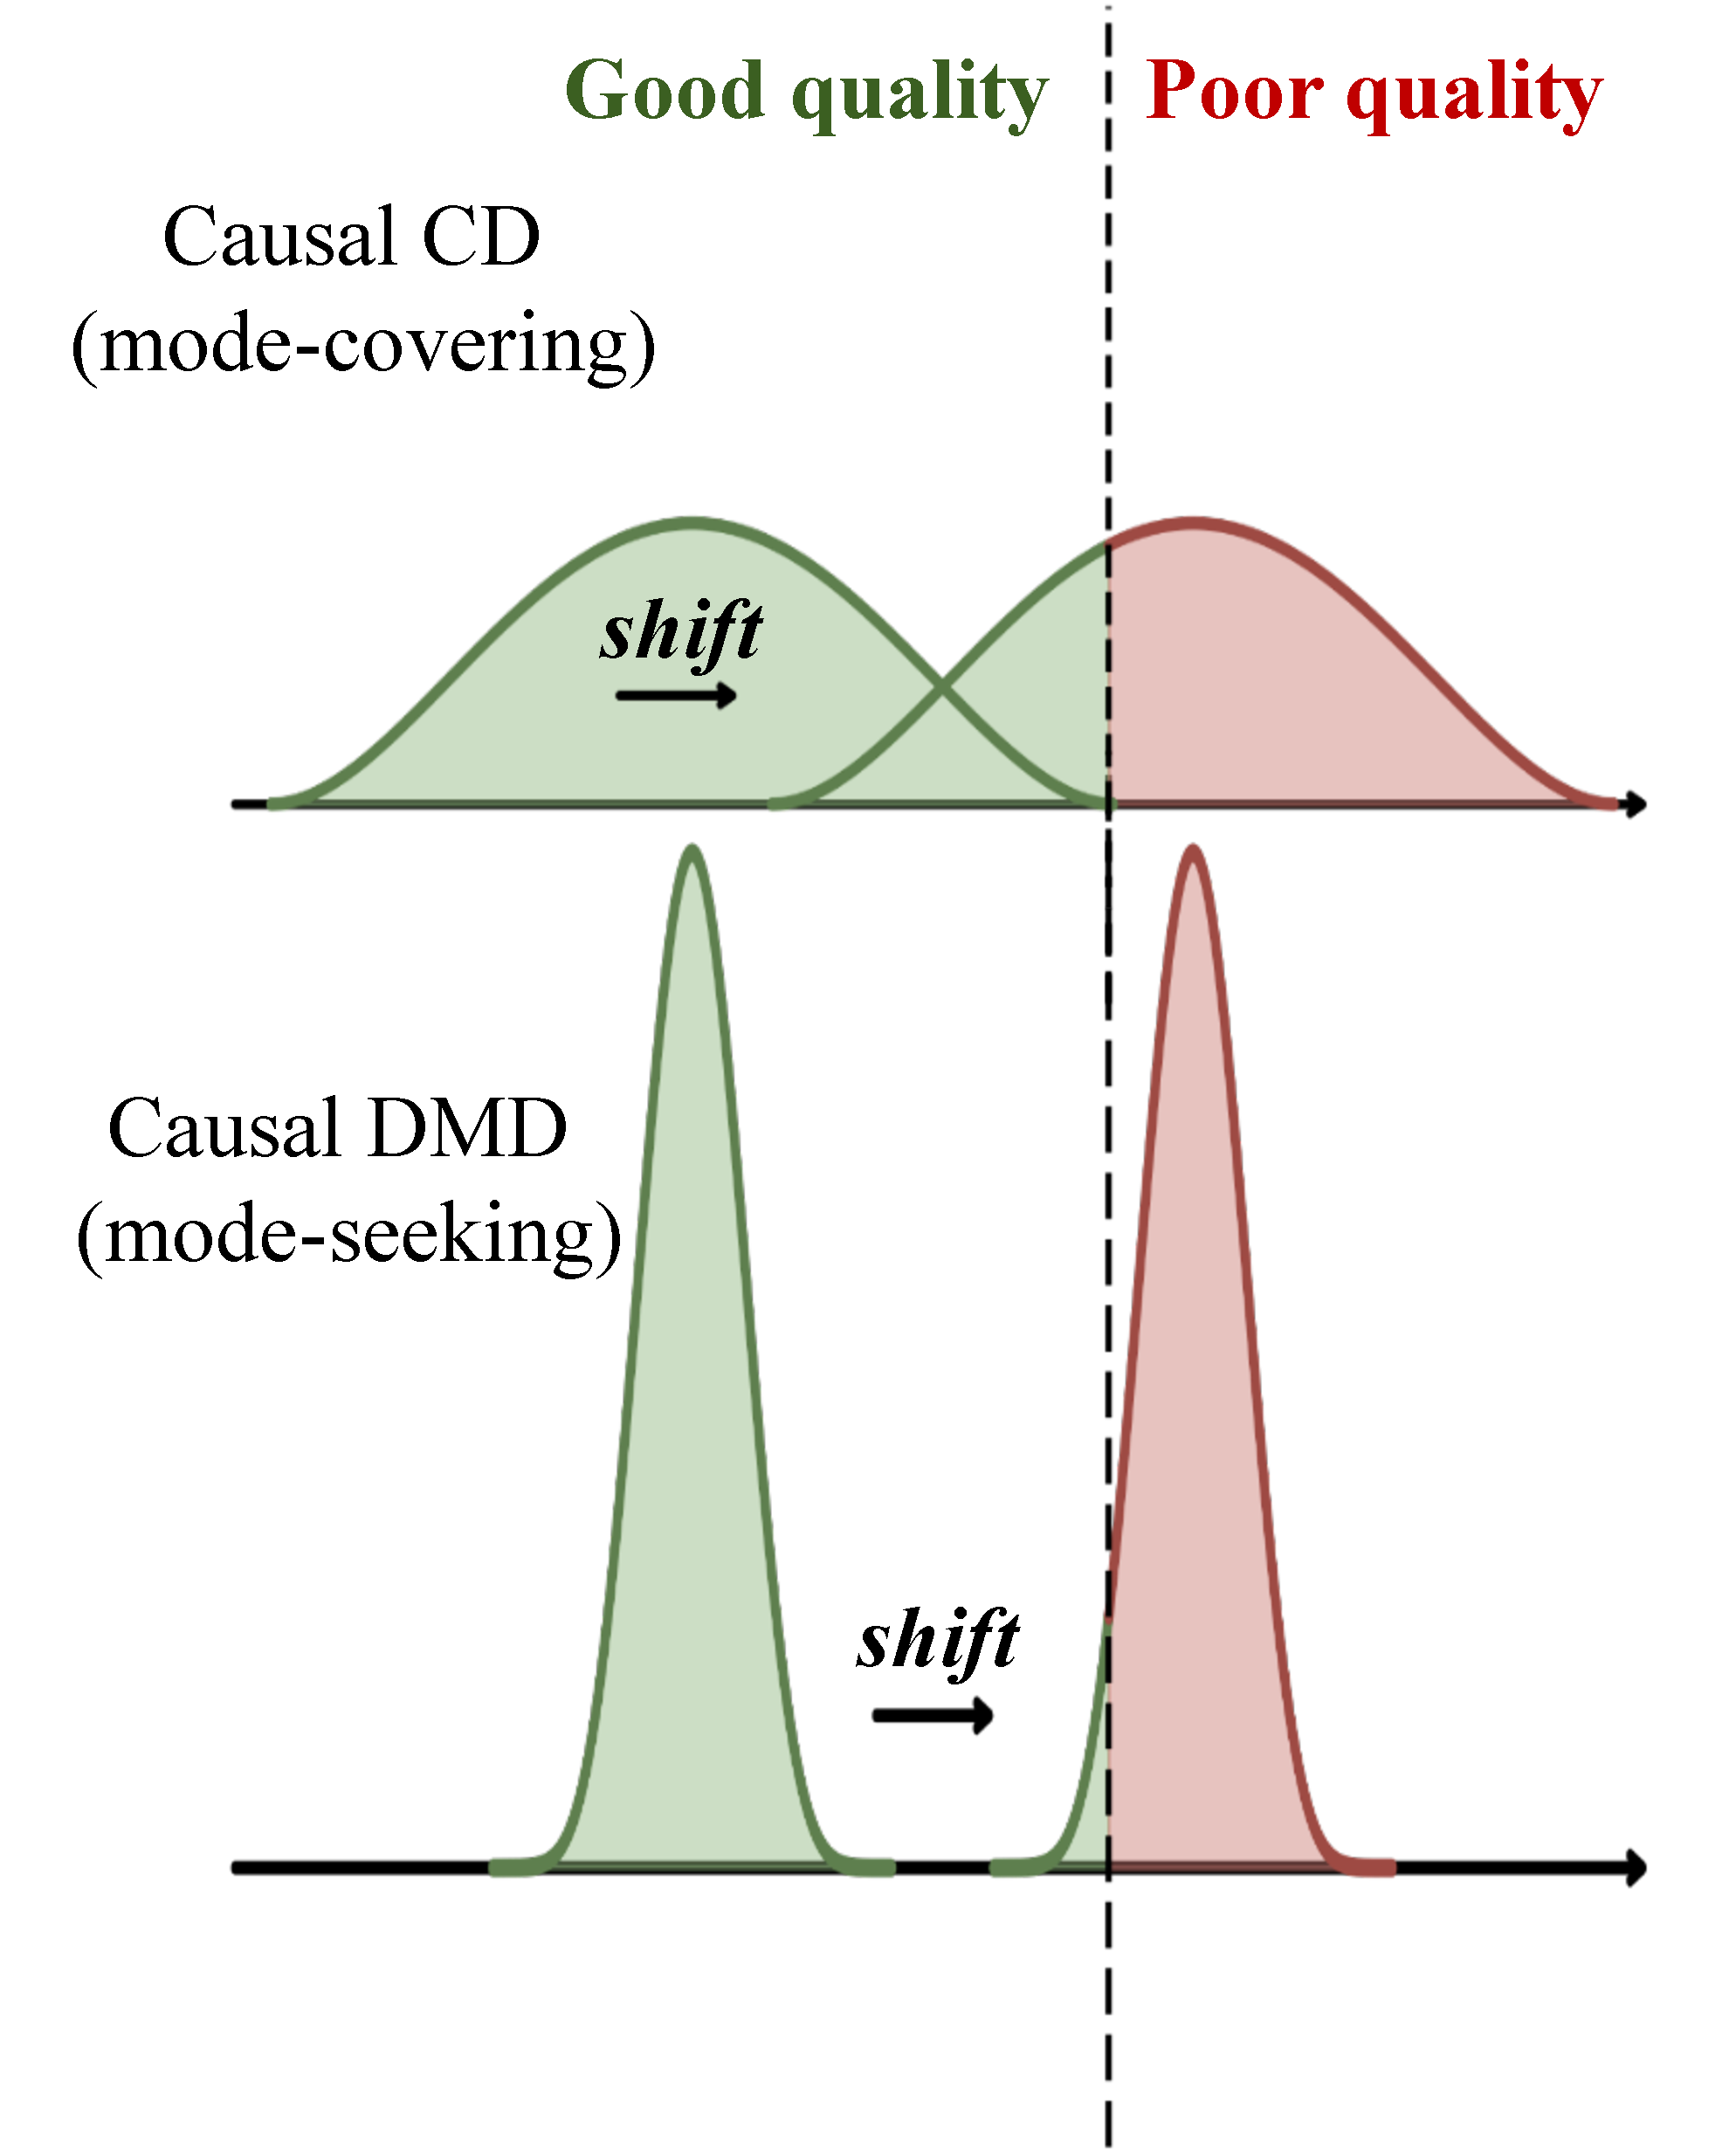
\includegraphics[width=1.25\linewidth]{Figures/causal-dmd-b.pdf}
    \caption{\footnotesize Under history shift, causal CD preserves good-quality mass; causal DMD shifts most mass into poor-quality regions.}
    \label{fig:causal-dmd-b}
  \end{subfigure}

  \caption{\textbf{Performance comparison between causal CD and causal DMD and the intuitive explanation.} Causal DMD achieves better early-frame quality than causal CD, but suffers from severe exposure bias in later frames, since mode-seeking DMD is more sensitive to accumulated errors.}
  \label{fig:dmd-is-worse-than-cd}
\end{figure}


\paragraph{Causal DMD with teacher forcing.} We begin by adapting score distillation into a teacher forcing causal form. Specifically, we take DMD~\cite{wang2023prolificdreamer,luo2023diff,yin2024one,yin2024improved} as a representative example and examine its causal variant. DMD optimizes the student generator through the gradient of the KL divergence between the noised student and data distributions. The student first produces $\tilde{\vx}\sim p_\theta(\tilde{\vx})$, which is then perturbed to $\tilde{\vx}_t$ through the forward diffusion process, inducing $p_{\theta,t}(\tilde{\vx}_t)$. A frozen diffusion model $s_{\text{real}}$ estimates the data score, while an online-trained diffusion model $s_{\text{fake}}$ estimates the student score. Their difference provides the distribution-matching direction, which is backpropagated to update the generator as follows:
\begin{align}
\label{eq:dmd}
\nabla_\theta\E_t[\KL(p_{\theta,t}(\tilde{\vx}_t)||p_{\text{data},t}(\tilde{\vx}_t))]
   = -\E_{\tilde{\vx}, t, \tilde{\vx}_t}[(s_\text{real}(\tilde{\vx}_t,t)-s_\text{fake}(\tilde{\vx}_t,t))\frac{\partial \tilde{\vx}}{\partial \theta}].
\end{align}
When distilling an AR diffusion model, the setting becomes slightly different: the teacher models $s_\text{real}$, $s_\text{fake}$ and the student $G_\theta$ all model conditional distributions autoregressively. Therefore, the above objective must be trained under teacher forcing, as follows:
\begin{align}
\label{eq:causal-dmd}
\nabla_\theta\E_t[\KL(p_{\theta,t}(\tilde{\vx}_t^i|\vx_{\mathrm{gt}}^{<i})||p_{\text{data},t}(\tilde{\vx}_t^i|\vx_{\mathrm{gt}}^{<i}))]
   = -\E_{\vx_{\mathrm{gt}}^{<i},\tilde{\vx}^i, t, \tilde{\vx}_t^i}[(s_\text{real}(\tilde{\vx}_t^i,\vx_{\mathrm{gt}}^{<i},t)-s_\text{fake}(\tilde{\vx}_t^i,\vx_{\mathrm{gt}}^{<i},t))\frac{\partial \tilde{\vx}^i}{\partial \theta}].
\end{align}
With this training scheme, we can directly distill an AR diffusion model via DMD into an AR few-step generator. Note that all models involved in causal DMD, including the teachers and the student, are autoregressive. It is therefore a purely causal distillation procedure, fundamentally different from the subsequent asymmetric DMD, where the teacher is bidirectional while the student is autoregressive. In summary, these two DMD stages serve distinct roles: causal DMD provides a few-step AR student initialization for the subsequent asymmetric DMD.

\paragraph{Severe exposure bias undermines causal DMD.}
Although bidirectional DMD usually achieves better quality than bidirectional CD~\cite{yin2024one,yin2024improved,zheng2025large}, we observe the opposite trend in the AR setting: causal DMD yields lower overall quality than causal CD, as shown by the Stage~2 VBench comparison in Fig.~\ref{fig:dmd-is-worse-than-cd}(a). More interestingly, this degradation is not uniform across frames. In the Stage~2 visualizations of Fig.~\ref{fig:dmd-is-worse-than-cd}(a), the first few frames generated by causal DMD even appear sharper and better than those from causal CD. However, as autoregressive generation proceeds, the later frames from causal DMD rapidly drift, accompanied by severe camera shifts, and eventually degrade to an unacceptable level. In contrast, although causal CD also suffers from gradual quality decay during autoregressive rollout, its degradation is far less severe. The Stage~3 results in Fig.~\ref{fig:dmd-is-worse-than-cd}(a) further show that using causal DMD as the initialization for the subsequent asymmetric DMD performs worse than using causal CD initialization. In summary, causal DMD suffers from substantially stronger exposure bias and is therefore unsuitable as a few-step initialization.

We further analyze why causal DMD can outperform CD in the first few frames but then rapidly suffers from amplified exposure bias, with an intuitive explanation illustrated in Fig.~\ref{fig:dmd-is-worse-than-cd}(b). As noted in prior work~\cite{zheng2025large}, DMD optimizes a reverse KL objective, whereas CD optimizes a forward KL objective. Compared with the mode-covering behavior induced by forward KL, the mode-seeking behavior of reverse KL tends to concentrate probability mass around high-density modes, leading to a sharper and less diverse distribution. This contrast is illustrated by the broader causal-CD distributions and the sharper causal-DMD distributions in Fig.~\ref{fig:dmd-is-worse-than-cd}(b). Early in autoregressive rollout, this concentration reduces the probability assigned to low-quality regions and thus improves generation quality, explaining the strong quality of the first few frames. However, such a concentrated distribution is also more sensitive to accumulated errors in autoregressive conditional generation.

Specifically, the arrows in Fig.~\ref{fig:dmd-is-worse-than-cd} denote the shift of the conditional distribution caused by history drift, i.e., the deviation of the self-generated prefix from the ground-truth history. Under such drift, the conditional distributions induced by both mode-covering causal CD and mode-seeking causal DMD shift toward the poor-quality region. For mode-seeking DMD, since the probability mass is highly concentrated, once the shifted mode moves into the poor-quality region, most generated samples tend to follow this erroneous mode, as shown by the shifted red DMD peak in Fig.~\ref{fig:dmd-is-worse-than-cd}(b). In contrast, mode-covering CD maintains a more dispersed distribution; even after the shift, a substantial portion of its probability mass can remain in the good-quality region, as shown by the broader shifted CD distribution in Fig.~\ref{fig:dmd-is-worse-than-cd}(b). Therefore, intuitively, mode-seeking DMD is more sensitive to accumulated history errors, causing exposure bias to rapidly amplify in later frames, whereas mode-covering CD suffers from exposure bias with much lower sensitivity.
